\namedsection{Machine Learning}{Playle}
\label{ml}

%%%%%%%%%%%%%%%%%%%%%%%%%%%%%%%%%
%%% WHAT IS MACHINE LEARNING? %%%
%%%%%%%%%%%%%%%%%%%%%%%%%%%%%%%%%
Machine learning is a technique that takes some observations about a system in addition to a value of interest \todo{Maybe s/value of interest/output/}, builds a model around these parameters and uses this model to create predictions about the value of interest for the system. There are typically three categories of machine learning algorithm: classification, where the value of interest is in a finite set of classes; regression, where the value of interest is continuous; and clustering, where the value of interest is related to other values.

In order to detect exercise, a classifying supervised machine learning algorithm will be most suitable, with the classes being types of activity observed.

\subsection{Considered Issues}

%%%%%%%%%%%%%%%%%%%%%%%%%%%%%%%
%%% CURSE OF DIMENSIONALITY %%%
%%%%%%%%%%%%%%%%%%%%%%%%%%%%%%%
One of the frequently encountered problems is the curse of dimensionality \cite{bellman1957dynamic}. Having a high number of dimensions, often as a result of having a large number of inputs into a machine learning algorithm, can create the problem whereby the amount of instances required to sufficiently train the model increases as the amount of training of the model must have instances such that the input feature space must be explored sufficiently. \cite{oommen2008objective}. Further to this effect, the time and space complexity of many machine learning algorithms are functions of the feature space's dimensionality. However, existing work has demonstrated that the curse of dimensionality is not necessarily applicable to time-series data as the nature of such data explores the feature space on the condition that the signal-to-noise ratio is sufficiently high \cite{bernecker2011quality}.

%%%%%%%%%%%%%%%%%%%
%%% OVERFITTING %%%
%%%%%%%%%%%%%%%%%%%
\todo{cites}
Another problem encountered in machine learning is that of overfitting, where the model for some algorithm is trained such that it specialises on the training set alone. This can be problematic where the model is introduced to new data, as such models have poor performance on unseen data. Overfitting can be prevented by reducing the complexity of the model, as if the model is not complex enough, it is not possible for it to overfit on the training data exactly. Additionally, evaluation should be performed on a data set other than the training set, which can be achieved with using cross-validation, or even having a completely separate data set on which to test.

\note{How exactly does the machine learning algorithm work? Reference papers that describe these methods.}

\note{What experiments were conducted in order to determine machine learning feasibility?}
\subsection{Initial Feasibility Assessment}
In order to initially determine the feasibility of applying machine learning for detecting exercise, a simple experiment was conducted with a single subject. The intent of the experiment was to implement a similar machine learning algorithm as is described in \cite{kwapisz2011activity} to ensure understanding of the problem at hand.

The collection device used came in the form of a Sony Z3 mobile phone, providing kinematic sensors, of which the gyroscope, measuring the angular velocity, was used. The subject had the collection device attached to their foot while they performed activities including a foot rotation exercise; walking on a flat surface; and walking up and down stairs. Additionally, noise was collected by moving the collection device in random directions. The collection device sampled data at 200Hz on each axis, so for the purpose of assessing feasibility, this value was carried through into machine learning, using a window size of 200 samples for a classification over 1 second intervals.

Data for each activity was collected separately to ensure classification could be performed without having to note exact timings of activities. Some examples of the data collected in these activities are shown in figure \ref{fig:first-data}, where the periodic nature of all the activities (with the exception of noise), can be seen clearly. \todo{Discuss this data more?}

This data was run through a series of tools to build a model, as described in section \ref{sec:tools-produced}. Initial evaluation of the performance was conducted using 10-fold cross-validation. The confusion matrix for a simple naive Bayes classifier is shown in table \ref{tab:first-confusion}, giving a classification accuracy of \todo{}. Despite the data only being collected from a single individual using a small set of instances, the results were promising, indicating that machine learning as a method of activity recognition was feasible.

\begin{table}[]
	\centering
	\begin{tabular}{|cccc|ll|}
		\hline
		\multicolumn{4}{|c|}{Classified As}   &          &                        \\
		Exercise & Noise & Stairs & Walking &          &                        \\
		\hline
		62       & 0     & 0      & 0       & Exercise & \multirow{4}{*}{Class} \\
		2        & 15    & 1      & 0       & Noise    &                        \\
		3        & 0     & 10     & 3       & Stairs   &                        \\
		1        & 0     & 1      & 7       & Walking  &                       \\
		\hline
	\end{tabular}
	\caption{Feasibility Assessment Confusion Matrix \label{tab:first-confusion}}
\end{table}


\begin{figure}
	\centering
	\subfigure[Exercise]{\label{fig:first-exercise}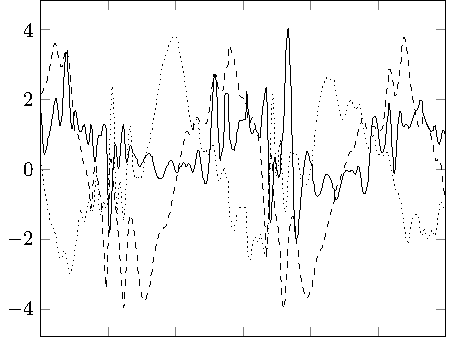
\includegraphics[width=70mm]{figures/first-exercise.pdf}}
	\subfigure[Noise]{\label{fig:first-noise}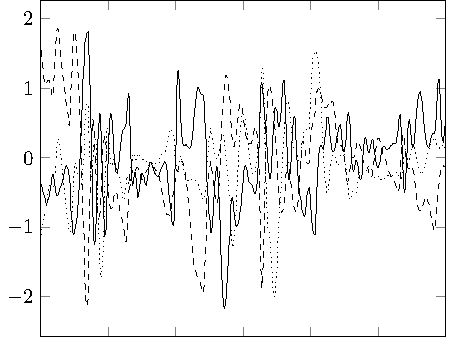
\includegraphics[width=70mm]{figures/first-noise.pdf}}
	\subfigure[Stairs]{\label{fig:first-stairs}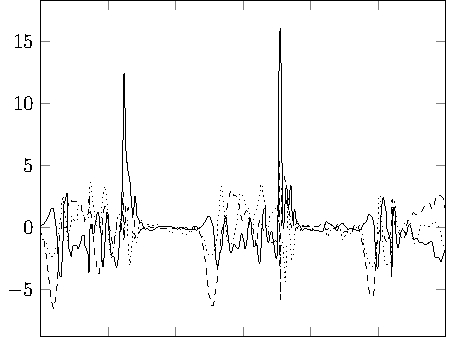
\includegraphics[width=70mm]{figures/first-stairs.pdf}}
	\subfigure[Walking]{\label{fig:first-walking}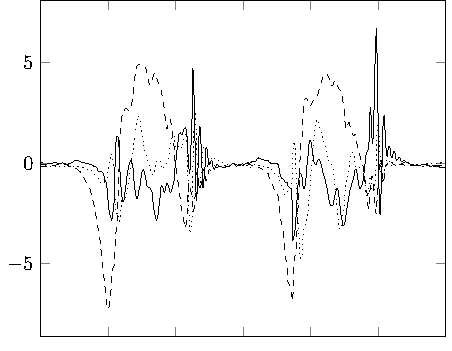
\includegraphics[width=70mm]{figures/first-walking.pdf}}
	\caption{Feasibility Assessment Data \label{fig:first-data}}
\end{figure}

%%%%%%%%%%%%%%%%%%%%%%%%%%%%%
%%% TOOLS USED / PRODUCED %%%
%%%%%%%%%%%%%%%%%%%%%%%%%%%%%
\subsection{Tools \label{sec:tools}}
Weka, a machine learning library, was used extensively for machine learning aspects. It provides a vast multitude of implemented machine learning algorithms, including various methods of evaluating the performance of these trained models.

%%%%%%%%%%%%%%%%%%%%%%%
%%% THE ARFF SCRIPT %%%
%%%%%%%%%%%%%%%%%%%%%%%
In order to produce this, it is first necessary to know the desired classification over given intervals for some time series data. This is achieved by mapping a single point of interest on some time series data to a class. This mapping is then passed to a script that takes windows centered on these points of interest and creates the corresponding \texttt{.arff}. In addition to these points of interest, the number of samples per window is also taken.

%%%%%%%%%%%%%%%%%%%%
%%% DOWNSAMPLING %%%
%%%%%%%%%%%%%%%%%%%%
Data collection is already an expensive task in terms of time consumed. It was therefore deemed infeasible to sample at multiple frequencies on top of all the variables being explored during data collection. Further to this, the device being used for data collection was rigid in terms of allowable sampling frequencies. To allow for analysis of multiple sampling frequencies at a later data, sampling was done at 200Hz, the fastest the collection device would allow. Any collected data could then be downsampled, which was achieved by taking the closest sample to $n/f$ where f is the frequency to downsample to.

%%%%%%%%%%%%%%%%%%%%%%
%%% CLASSIFICATION %%%
%%%%%%%%%%%%%%%%%%%%%%
As shown in figure \ref{fig:first-data}, activities produce periodic data that is easily manually identified. This feature of the collected data was used to in order to identify the intervals for classification. Collected data was separated at the time of collection into individual files each representing a different activity/sensor tuple, allowing for trivial manual classification.

The act of data classification occurred by viewing the plotted data and points of interest were noted. For the two exercise classes \todo{Name the classes?}, the points of interest were the peak and trough of the y-axis. For the class representing not exercise, points of interest were taken at frequent points throughout collected data files where subjects were not performing exercise, meaning that manual classification of the not exercise class was not required.

These classified points of interest were then run through a script 

%%%%%%%%%%%%%%%%%%%%%%%%%%%%%%%%%%%
%%% ASSESSING MODEL PERFORMANCE %%%
%%%%%%%%%%%%%%%%%%%%%%%%%%%%%%%%%%%
There are multiple methods of assessing the performance of a model. A simple assessment may include measuring the accuracy, although this does not take into account the probability of specific classes existing, and can therefore skew results when there are significantly more instances of a subset of classes over another subset of classes. An extreme example of this is the 0-R classifier, which will determine the most frequent class and classify all instances as this. Such a classifier is very simple, and has a severely limited utility, but as shown in \todo{figure}, a high accuracy is still possible, despite what can be considered poor performance.

By taking into account the probability of classes existing, the bias that leads to this poor metric can be eliminated. Such a statistic is the kappa statistic \todo{add cite}, which measures performance with respect to a null classifier, that is, a classifier that solely takes into account the frequencies of observed data. A kappa statistic, $\kappa < 0$  would indicate very bad performance (worse than guessing while taking into account the class frequencies). $\kappa$ increasing from 0 to 1 indicates increasing performance, with $\kappa = 1$ being a perfect classifier. The kappa statistic has therefore been used to measure the performance of later classifiers.

% Maybe remove this
In some cases, it may be important to quantify the trade-off a classifier makes between true and false positives. This can especially be the case where it is more important to detect some class over another. Achieving this can be done with a custom cost function, which is applied to the resultant confusion matrix (equation \ref{eq:cost}). From this, the average cost per instance can be computed, allowing comparisons to be drawn.

\begin{equation}
	\label{eq:cost}
	\begin{gathered}
		\text{Cost } c = \langle \mathbf{COST}, \mathbf{CONFUSION} \rangle_F \\
		\text{Where $\langle \mathbf{A}, \mathbf{B}\rangle_F$ is the Frobenius inner product between $\mathbf{A}$ and $\mathbf{B}$}
	\end{gathered}
\end{equation}

This method of performance quantification is similar to an ROC curve, except where 

Weka accepts instances in the form of an \texttt{.arff} file, this file specifies all the classes for the classifier to accept; the inputs for the classifier; and some number of instances and their actual class, if known.


%%%%%%%%%%%%%%%%%%%%%%%%%%%%%
%%% 3 CLASSES OVER JUST 2 %%%
%%%%%%%%%%%%%%%%%%%%%%%%%%%%%
The number of classes to classify was considered, as a variable parameter for the classifier. A classifier with the 2 classes \textit{exercise} \todo{Maybe s/exercise/activity/} and \textit{not exercise}, would only allow for binary classification. Depending on the classifier behaviour and the nature of the exercise in question, it may be the case that when the window of classification lies between 2 exercises, the window could be classified as either class. This unpredictable behaviour would prevent further analysis of the subject's exercise beyond how much time exercise has been detected for. \todo{Add figure}. However, by splitting the \textit{exercise} class into 2 distinct classes, such that every exercise performed will always be composed of these parts, it allows 3 classes to be used with the classifier. Such a change would allow counting of distinct exercises, by ensuring that one type of \textit{exercise} class is followed by the other type of \textit{exercise} class. This would allow the number of exercises to be counted, as well as the amount of time exercised. Further to this, the additional information may allow for heuristics to increase accuracy should the classifier ``bounce''. \todo{More on this in heuristics...} Other numbers of classes were also considered, such as some number of classes for the exercise, along with a class for each likely type of non-exercise activity. \todo{and this idea was rejected because...}

\note{What classification algorithms were trialled? What kind of results were achieved with these. Explain and discuss the workings of each algorithm / type of algorithm.}

\subsection{Multilayer Perceptrons}
A Multilayer Perceptron (MLP) is a type Neural Network, where the nodes, or perceptrons, are organised in layers. Each node accepts some number of inputs with some weight. These summation of these weighted inputs are computed and applied to some activation function, the result of which is the output of the node (equation \ref{eq:perceptron}).

\begin{equation}
\label{eq:perceptron}
\text{Output } o = activation\bigg(\sum_{i=1}^{d}{x_iw_i}\bigg) 
\end{equation}

Each perceptron affectively defines a plane in $d$-dimensional space. Instances on either side of this plane can then be classed, allowing a single perceptron to act as a simple classifier. By combining multiple perceptrons in a layer, it is possible to build up these planes in order to create more complex classifier made of these linear classifiers. The addition of layers, using previous layers are inputs allows a more complex classifier still by allowing the importance of these sub-classifiers to vary with the inputs. MLPs with enough inputs and layers can therefore replicate any function \cite{baum1988capabilities}.

\begin{figure}
	\centering
	% I'm not too happy with this, but it'll do, I guess...
	\begin{tikzpicture}[shorten >=1pt,node distance=1.3cm and 3cm,on grid,auto,initial text={}] 
	\node[state,rectangle] (i1) {$i_1$};
	\node[state,rectangle] (i2) [below=of i1] {$i_2$}; 
	\node[state,rectangle] (in) [below=of i2] {$i_n$}; 
	
	\node[state] (h11) [right=of i1] {$h_{1,1}$};
	\node[state] (h12) [below=of h11] {$h_{1,2}$}; 
	\node[state] (h1a) [below=of h12] {$h_{1,a}$}; 
	
	\node[state] (hb1) [right=of h11] {$h_{b,1}$};
	\node[state] (hb2) [below=of hb1] {$h_{b,2}$}; 
	\node[state] (hba) [below=of hb2] {$h_{b,a}$}; 
	
	\node[state] (o) [right=of hb2] {$o$};
	\path[->] 
	(i1) edge node {} (h11) (i2) edge node {} (h11)
	(i1) edge node {} (h12) (i2) edge node {} (h12)
	(i1) edge node {} (h1a) (i2) edge node {} (h1a)
	(in) edge node {} (h11) (h11) edge node {} (hb1)
	(in) edge node {} (h12) (h11) edge node {} (hb2)
	(in) edge node {} (h1a) (h11) edge node {} (hba)
	(h12) edge node {} (hb1) (h1a) edge node {} (hb1)
	(h12) edge node {} (hb2) (h1a) edge node {} (hb2)
	(h12) edge node {} (hba) (h1a) edge node {} (hba)
	
	(hb1) edge node {} (o)
	(hb2) edge node {} (o)
	(hba) edge node {} (o)
	;
	\end{tikzpicture}
	\caption{Example topology of a MLP \label{fig:mlp-topology}}
\end{figure}

\subsection{Radial Basis Function Networks}
A Radial Basis Function (RBF) network is a type of Neural Network that is composed of 2 layers, an input layer and an output layer. The activation functions for this output layer are RBFs. An RBF can be any function that is only dependent on the distance from some point. An example of a commonly used RBF is the Gaussian function.

\subsection{Instance-Based Learning}
Instance-based learning is a type of machine learning algorithm that postpones model creation until an output for a problem instance is required. Some number of labelled instances are stored in memory, and these are used to label problem instances.

Instance-based learning is advantageous over other machine learning methods in that adapting the model with new instances is trivial. This makes it attractive for simple systems where some adaptation of the model is required.

As a number of labelled instanced must be kept in memory in order to compute the model, instance-based learning methods can require large amounts of memory to classify. Additionally, any problem instances must be compared against each labelled instanced that is to be used for the model, meaning that time complexity for classification of any problem instance is linear in the number of labelled instances. This can present significant challenges when the size of the training data set become large with respect to the underlying device.

An example of instance-based learning is the k-nearest neighbours algorithm where any problem instance is compared to the k-nearest labelled instances. The class that the problem instance is most similar to is then given this classification. \todo{Reword}

\note{What issues were faced as a result of implementing a machine learning algorithm on a constrained system? How were these problems overcome? \cite{anguita2012human}}
Each machine learning algorithm comes with its own memory-processing-accuracy trade-off, 

%%%%%%%%%%%%%%%%%%%%%%%%%%%%
%%% ALGORITHM PARAMETERS %%%
%%%%%%%%%%%%%%%%%%%%%%%%%%%%
\note{Selection of the algorithm - mention hidden layers  /frequency}
There are many parameters that affect the performance of classifiers. In the case of the collected data, the sampling frequency for the kinematic sensor and the window with a number of samples over which the classifier classifies have a direct impact on the classifier's ability to perform. In the case of the model, most machine learning algorithms have some form parameters allowing their behaviour to change. 

As the MLP was 

%%%%%%%%%%%%%%%%%%%%%%%%%%
%%% USER STUDY RESULTS %%%
%%%%%%%%%%%%%%%%%%%%%%%%%%
\subsection{User Study Results}
\note{As a result of the user study, how did the results change? Note observed results due to the user study.}
The user study was performed on a number \todo{How many?} subjects, where both accelerometer and gyroscope data was collected for multiple activities.

%%%%%%%%%%%%%%%%%%%%%%%%%%%
%%% ALGORITHM SELECTION %%%
%%%%%%%%%%%%%%%%%%%%%%%%%%%
The main contenders for the algorithm were the MLP and RBF network due to high performance while having relatively low complexity, allowing them to be implemented on a constrained device without too much difficulty. Between these two algorithms, there was minimal difference in terms of 

\begin{figure}
	\centering
	\subfigure[Top-Down]{\label{fig:mlp-multi-flat}\includegraphics[width=70mm]{figures/mlp-multi-analysis-flat.pdf}}
	\subfigure[Side-On, Varying Hidden Layers]{\label{fig:mlp-multi-3d}\includegraphics[width=64mm]{figures/mlp-multi-analysis-3d.pdf}}
	%\subfigure[Varying Frequency]{\label{fig:mlp-multi-3d-2}\includegraphics[width=70mm]{figures/mlp-multi-analysis-3d-2.pdf}}
	%\subfigure[Varying Both]{\label{fig:mlp-multi-3d-3}\includegraphics[width=70mm]{figures/mlp-multi-analysis-3d-3.pdf}}
	\caption{MLP Parameter Performance Surface Plot \label{fig:mlp-multi}}
\end{figure}

\begin{figure}
	\includegraphics[width=\linewidth]{subject-fold-results.pdf}
	\caption{Subject Performance with Different Sensors and Algorithms \label{fig:subfold}}
\end{figure}

%%%%%%%%%%%%%%%%%%%%%%%%%%%%%%%%%%%
%%% WHY CROSS-VALIDATION IS BAD %%%
%%%%%%%%%%%%%%%%%%%%%%%%%%%%%%%%%%%
To evaluate the models on the user study data, cross-validation was considered, as this would allow training on some set of data and then testing on another set previously unseen to the model, although this would have the slightly undesirable effect of mixing data from subjects, whereas in practice, the device will be trained on a set of subjects and used by a subject not in that set. To replicate this kind of behaviour, a similar method to cross-validation was used, where the model was trained on all subjects, except for one. This one excluded subject was then tested on. This method is then repeated for all subjects. This subject-fold cross-validation method is also beneficial in allowing conclusions to be drawn about subject performance in relation to other subjects.

%%%%%%%%%%%%%%%%%%%%%%%%%%%
%%% SUBJECT PERFORMANCE %%% Woo, statistics!
%%%%%%%%%%%%%%%%%%%%%%%%%%%
Figure \ref{fig:subfold} shows the resultant performance, measured using the kappa statistic, for each of the subjects performing activities using different sensors sampling at 20Hz for the MLP and RBF classifiers. These results are collected using the subject-fold cross-validation technique as previously described. \todo{Could mention accl and gyro data collected independently.}. As the \textit{Accelerometer using MLP} result class is likely to require the most suitable for a low-power constrained device \todo{As mention in ...}, this shall be used as a base-line to compare performance against. The null hypothesis was the mean of other result classes were equal to the mean of \textit{Accelerometer using MLP}. The alternative hypothesis was that these means were different. These hypothesises were tested using a series of \textit{t}-tests with significance level, $\alpha = 0.01$. The resultant $p$-values from these $t$-tests are displayed in table \ref{tab:res-ttest}. Despite the \textit{Gyroscope using MLP} and \textit{Accelerometer using RBF} result classes having a higher mean performance than \textit{Accelerometer using MLP} class, these increases were not statistically significant and therefore the null hypothesis in these cases could not be rejected. For \ textit{Gyroscope using RBF}, a statistically significant change in mean performance was observed, leading to acceptance of the alternative hypothesis.

\begin{table}
	\centering
	\begin{tabular}{l|ll}
		& Mean Performance & $p$-value \\
		\hline
		Accelerometer using MLP & 0.5842 & N/A \\
		Gyroscope using MLP     & 0.6204 & 0.6054 \\
		Accelerometer using RBF & 0.6116 & 0.5858 \\
		Gyroscope using RBF     & 0.8016 & $2.064 \times 10^{-4}$ \\        
	\end{tabular}
	\caption{Result classes statistical significance \label{tab:res-ttest}}
\end{table}

A noteworthy observation about the results was that the performance of the algorithm was initially poor, by any measure, after the first day data collection, giving just 5 \todo{Really?} subjects to model against. However, as the number of subjects increased, so did the performance of the system. This would indicate that the algorithm was overfitting on subjects, and that the introduction of more subjects was able to at least in part negate this overfitting.

\note{What parameters are there and how did they affect the accuracy of the system?}

\note{Still need to add RBF stuff...}